\documentclass[border=6pt]{standalone}
\usepackage{amsmath,amssymb}
\usepackage{tikz}
\usetikzlibrary{arrows.meta,shadows,calc,backgrounds}
\begin{document}
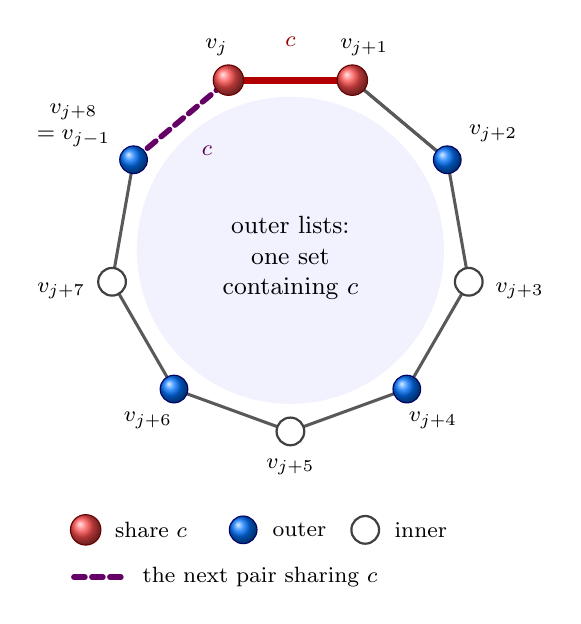
\begin{tikzpicture}[
  outer/.style={circle,inner sep=0pt,minimum size=10pt,ball color=blue!55!cyan,draw=blue!40!black,line width=0.4pt},
  inner/.style={circle,inner sep=0pt,minimum size=10pt,draw=black!75,line width=0.8pt,fill=white},
  pair/.style={circle,inner sep=0pt,minimum size=11pt,ball color=red!70,draw=red!40!black,line width=0.4pt},
  pe/.style={line width=1.1pt,black!65},
  shared/.style={line width=2.6pt,red!70!black,line cap=round},
  next/.style={line width=2.0pt,violet!80!black,dash pattern=on 4pt off 2.5pt,line cap=round},
  lab/.style={font=\footnotesize}]
\def\R{2.3}
% vertex v_{j+i} at angle 110 - 40 i
\foreach \i in {0,...,8} { \coordinate (u\i) at ({110-40*\i}:\R); }
\begin{scope}[on background layer]
  \fill[blue!5] (0,0) circle (\R-0.35);
\end{scope}
\foreach \i [evaluate=\i as \j using int(\i+1)] in {1,...,7} { \draw[pe] (u\i) -- (u\j); }
\draw[shared] (u0) -- (u1);
\draw[next] (u8) -- (u0);
\draw[pe] (u1) -- (u2);
\node[pair] at (u0) {};
\node[pair] at (u1) {};
\foreach \i in {2,4,6,8} { \node[outer] at (u\i) {}; }
\foreach \i in {3,5,7} { \node[inner] at (u\i) {}; }
% labels
\node[lab,anchor=290] at ($(u0)+(110:0.2)$) {$v_j$};
\node[lab,anchor=250] at ($(u1)+(70:0.2)$) {$v_{j+1}$};
\foreach \i in {2,...,7} { \node[lab,anchor={290-40*\i}] at ($(u\i)+({110-40*\i}:0.22)$) {$v_{j+\i}$}; }
\node[lab,align=center,anchor=330] at ($(u8)+(150:0.2)$) {$v_{j+8}$\\ $=v_{j-1}$};
\node[lab,red!60!black] at ({90}:{\R+0.35}) {$c$};
\node[lab,violet!70!black] at ({130}:{\R-0.65}) {$c$};
\node[font=\small,align=center] at (0,-0.1) {outer lists:\\ one set\\ containing $c$};
% legend
\node[pair] at (-2.6,-3.55) {}; \node[lab,anchor=west] at (-2.35,-3.55) {share $c$};
\node[outer] at (-0.6,-3.55) {}; \node[lab,anchor=west] at (-0.35,-3.55) {outer};
\node[inner] at (0.95,-3.55) {}; \node[lab,anchor=west] at (1.2,-3.55) {inner};
\draw[next] (-2.75,-4.15) -- (-2.15,-4.15); \node[lab,anchor=west] at (-2.0,-4.15) {the next pair sharing $c$};
\end{tikzpicture}
\end{document}
